\section{Разработка программных модулей}
\subsubsection{Развёртывание \textit{Kubernetes} кластера через \textit{Ansible} и \textit{GitLab CI/CD}.} Процесс развёртывания  кластера организован с помощью инфраструктурного кода, исполняемого в пайплайне \textit{GitLab CI/CD}. Ниже перечислены основные шаги, выполняемые в рамках автоматизации:

\begin{itemize}
  \item инициализация \textit{CI/CD}пайплайна с тремя стадиями: \lstinline{lint}, \lstinline{test} и \lstinline{deploy};
  \item подготовка \textit{bootstrap}-узла вручную с использованием пароля и плейбука \lstinline{bootstrap.yaml};
  \item применение базовой конфигурации через плейбук \lstinline{base-node.yaml}, создающий пользователей и настраивающий окружение;
  \item установка и конфигурация \textit{Kubernetes} с помощью плейбука \lstinline{k3s.yaml}, разделённого по ролям на \textit{master}- и \textit{agent}-узлы;
  \item использование переменных окружения и \textit{Ansible Vault} для безопасного хранения секретов;
  \item проверка и применение изменений происходит в пайплайне \textit{GitLab} при помощи \textit{dry-run} и ручного деплоя.
\end{itemize}

\subsubsection{Инициализация \textit{CI/CD}-пайплайна.} В \lstinline{.gitlab-ci.yml} определены три стадии пайплайна:

\begin{lstlisting}
stages:
  - lint
  - test
  - deploy
\end{lstlisting}

На стадии \lstinline{lint} выполняется статическая проверка \textit{playbook}'ов с помощью \lstinline{ansible-lint}. На стадии \lstinline{test} все плейбуки запускаются в режиме проверки (\lstinline{--check --diff}), без внесения изменений. На стадии \lstinline{deploy} \textit{playbook}'и применяются на удалённых узлах.

\subsubsection{Подготовка bootstrap-узла.} Этот шаг выполняется вручную, с помощью команды в пайплайне:

\begin{lstlisting}
ansible-playbook playbooks/bootstrap.yaml -i "${BOOTSTRAP_HOST}," \
  --user "${BOOTSTRAP_USER}" \
  --connection-password-file .bootstrap-root-password
\end{lstlisting}

На этом этапе развёртывается роль \lstinline{bootstrap}, которая выполняет начальную настройку: доступ по \textit{SSH}, установка базовых зависимостей и подготовка к следующему этапу.

\subsubsection{Применение базовой конфигурации.} Следующий шаг -- конфигурация базового окружения на всех нодах с помощью:

\begin{lstlisting}
ansible-playbook playbooks/base-node.yaml -l all
\end{lstlisting}

Этот плейбук настраивает пользователей, \textit{SSH}-ключи, группы, \textit{sudo}-доступ и другие параметры для дальнейшего управления нодами через \textit{Ansible}.

\subsubsection{Установка и настройка \textit{Kubernetes}.} Установка и настройка кластерного программного обеспечения\cite{k3s} осуществляется с помощью плейбука \lstinline{k3s.yaml}. Внутри него используются следующие роли:

\begin{itemize}
  \item \lstinline{k3s_server} -- применяется к мастер-нодам;
  \item \lstinline{k3s_agent} -- применяется к агентам;
  \item \lstinline{prereq} -- обрабатывает все узлы и подготавливает их к установке.
\end{itemize}

\subsubsection{Роль \textit{prereq} -- подготовка всех узлов кластера.}
Роль \textit{prereq} служит для подготовки узлов перед установкой и запуском кластера \textit{k3s}. Основная задача —- обеспечить выполнение всех системных требований и настроек, необходимых для корректной работы \textit{k3s} на каждом узле. В рамках этой роли производится проверка окружения, установка обязательных пакетов и настройка системных параметров.

В ходе выполнения роли выполняются следующие основные действия:
\begin{itemize}
  \item проверяется соответствие версии \textit{Ansible} минимальному требованию (не ниже \textit{2.14});
  \item устанавливаются зависимости: \textit{policycoreutils} для \textit{Ubuntu}, \textit{nfs-utils} для \textit{RHEL}-совместимых дистрибутивов, \textit{nfs-common} для \textit{Ubuntu};
  \item активируется \textit{IP}-маршрутизация: параметр \textit{net.ipv4.ip\_forward} включается всегда, \textit{IPv6}-маршрутизация включается при наличии \textit{IPv6}-адресов;
  \item собираются системные факты, включая сведения о брандмауэрах;
  \item при наличии активного \textit{ufw} открываются необходимые порты для \textit{API}-сервера и \textit{etcd}.
\end{itemize}

Таким образом, роль \textit{prereq} гарантирует, что все узлы имеют необходимое программное обеспечение и системные настройки для успешного развертывания и функционирования кластера \textit{k3s}.

\subsubsection{Роль \textit{k3s\_server} -- установка и настройка управляющих узлов.}
Роль \textit{k3s\_server} отвечает за установку и конфигурирование управляющих (\textit{control plane}) узлов кластера \textit{k3s}. Управляющие узлы обеспечивают работу \textit{API}-сервера, управления состоянием кластера и координацию работы рабочих узлов. В зависимости от архитектуры кластера (один управляющий узел или несколько в режиме \textit{HA}) процесс установки и настройки имеет некоторые отличия.

В процессе выполнения роли происходят следующие этапы:
\begin{itemize}
  \item определяется текущая установленная версия \textit{k3s};
  \item при отсутствии или несоответствии версии загружается установочный скрипт и выполняется установка без автозапуска;
  \item добавляется автодополнение \textit{k3s} в \textit{.bashrc} пользователя;
  \item при наличии \textit{YAML}-конфига он копируется в \textit{/etc/rancher/k3s/config.yaml};
  \item если узел является первым в списке управляющих, выбирается соответствующий шаблон \textit{systemd}-юнита, прописываются переменные окружения, запускается сервис и выполняется настройка \textit{kubeconfig};
  \item если узел не первый, используется шаблон для режима \textit{HA} или с внешней БД, запускается сервис и проверяется присоединение узла к кластеру;
  \item при включённой опции настройки пользователя создаётся символьная ссылка \textit{kubectl}, настраивается каталог \textit{\textasciitilde/.kube}, копируется \textit{kubeconfig} и добавляется автозагрузка переменной окружения \textit{KUBECONFIG}.
\end{itemize}

В итоге роль \textit{k3s\_server} обеспечивает корректное развёртывание управляющей части кластера, её запуск и подготовку необходимых инструментов для управления кластером.

\subsubsection{Роль \textit{k3s\_agent} -- установка и настройка рабочих узлов.}
Роль \textit{k3s\_agent} предназначена для установки и настройки рабочих (\textit{worker}) узлов, которые выполняют контейнеры и предоставляют вычислительные ресурсы кластера. Для корректной работы рабочих узлов необходимо обеспечить их надёжное подключение к управляющим узлам и синхронизацию конфигурации.

Основные шаги, реализуемые в рамках роли:
\begin{itemize}
  \item определяется установленная версия \textit{k3s};
  \item при необходимости загружается установочный скрипт и запускается установка с параметром \textit{INSTALL\_K3S\_EXEC=agent};
  \item при изменении токена старое значение удаляется из файла окружения;
  \item актуальный \textit{K3S\_TOKEN} сохраняется в переменной окружения;
  \item копируется \textit{systemd}-юнит \textit{k3s-agent.service};
  \item сервис \textit{k3s-agent} активируется и запускается.
\end{itemize}

Таким образом, роль \textit{k3s\_agent} обеспечивает автоматизированное развёртывание рабочих узлов, их подключение к управляющим и подготовку к выполнению задач внутри кластера.

Для запуска роли на мастерах:

\begin{lstlisting}
ansible-playbook playbooks/k3s.yaml -l k8s_masters
\end{lstlisting}

Для запуска на агентах:

\begin{lstlisting}
ansible-playbook playbooks/k3s.yaml -l k8s_agents
\end{lstlisting}

Конфигурация передаётся через переменные, включая версию \textit{k3s}, сетевые параметры и \textit{TLS}-настройки.

\subsubsection{Управление секретами и переменными.} Все чувствительные данные, такие как пароли, ключи \textit{SSH} и токены, передаются через переменные окружения в \textit{GitLab} и \textit{Ansible Vault}. В пайплайне используется следующая логика декодирования:

\begin{lstlisting}
echo "${SSH_PRIVATE_KEY}" | base64 -d > ~/.ssh/id_rsa
echo "${VAULT_TOKEN}" > .vault-password
\end{lstlisting}

\textit{Vault} используется для расшифровки зашифрованных данных в плейбуках и переменных, что позволяет безопасно хранить ключи и пароли в репозитории.

\subsubsection{Проверка и развёртывание изменений.} На стадии \lstinline{test} выполняется \textit{dry-run} всех плейбуков с помощью:

\begin{lstlisting}
ansible-playbook --check --diff playbooks/${PLAYBOOK} -l ${LIMIT}
\end{lstlisting}

На стадии \lstinline{deploy} происходит фактическое применение:

\begin{lstlisting}
ansible-playbook playbooks/${PLAYBOOK} -l ${LIMIT}
\end{lstlisting}

Для последовательного применения нескольких плейбуков используется \lstinline{matrix} в \textit{GitLab CI}:

\begin{lstlisting}
.parallel.playbooks:
  parallel:
    matrix:
      - PLAYBOOK:
          - base-node.yaml
          - minio.yaml
          - k3s.yaml
\end{lstlisting}

Это обеспечивает возможность масштабируемого и контролируемого развёртывания.


\subsection{Обоснование использования \textit{Helm}}

\textit{Helm} -- это инструмент управления пакетами для \textit{Kubernetes}, который позволяет автоматизировать развертывание приложений, их обновление и управление ими. \textit{Helm} упрощает процесс создания, настройки и деплоя приложений в \textit{Kubernetes}, обеспечивая стандартизированные и удобные механизмы для работы с конфигурациями. Использование \textit{Helm} становится удобным в рамках \textit{CI/CD}процессов, особенно когда требуется быстро развертывать и управлять сложными микросервисными архитектурами.

Основным понятием \textit{Helm} является так называемый чарт (\textit{Helm Chart}). Чарт представляет собой набор файлов, которые описывают все необходимые ресурсы \textit{Kubernetes} для развертывания приложения. Это включает в себя такие компоненты, как деплойменты, сервисы, инграсы и другие объекты \textit{Kubernetes}. Каждый чарт состоит из нескольких файлов, среди которых важнейшими являются файлы шаблонов (\textit{templates}) и файл конфигурации \textit{values.yaml}.

\textit{Helm} использует мощную систему шаблонов для генерации манифестов \textit{Kubernetes}. Шаблоны в \textit{Helm} определяются с помощью языка \textit{Go}-шаблонов. Эти шаблоны позволяют динамически генерировать конфигурации на основе переменных, условий и других параметров. Шаблоны \textit{Helm} содержат стандартные элементы \textit{Kubernetes} манифестов, такие как \textit{Deployment}, \textit{Service}, \textit{ConfigMap} и другие ресурсы. 

Шаблоны в \textit{Helm} предоставляют несколько ключевых возможностей:

\begin{enumerate}
    \item \textit{Переменные и параметры}. Шаблоны могут включать переменные, которые определяются в файле \textit{values.yaml} или передаются во время установки \textit{Helm}-чарта. Это позволяет создавать гибкие конфигурации, которые можно адаптировать под разные окружения или потребности, например, изменять количество реплик, название контейнера или используемые порты.
    \item \textit{Условные операторы}. Шаблоны могут включать условные конструкции (\textit{if}, \textit{else}), которые позволяют в зависимости от значений переменных менять поведение шаблона. Например, можно условно подключать дополнительные сервисы или изменять параметры конфигурации в зависимости от среды (разработка, тестирование, продакшн).
    \item \textit{Циклы}. Шаблоны \textit{Helm} поддерживают циклические конструкции (\textit{range}), что позволяет автоматически генерировать одинаковые блоки конфигурации, например, для нескольких реплик подов или нескольких сервисов.
    \item \textit{Функции}. В шаблонах \textit{Helm} можно использовать встроенные функции, такие как \textit{lookup}, \textit{toYaml}, \textit{toJson}, \textit{default}, которые позволяют манипулировать данными и генерировать более сложные конфигурации.
\end{enumerate}

Шаблоны позволяют эффективно управлять различными аспектами развертываемого приложения и легко адаптировать его под изменяющиеся требования, что делает \textit{Helm} мощным инструментом для работы с \textit{Kubernetes}.

Файл \textit{values.yaml} играет ключевую роль в конфигурировании \textit{Helm}-чарта. Это файл, в котором задаются значения для переменных, используемых в шаблонах. Он позволяет централизованно управлять настройками приложения, не меняя напрямую шаблоны. Все параметры, такие как количество реплик, образ контейнера, порты и другие, определяются в \textit{values.yaml}, что делает процесс настройки более удобным и гибким. Эти значения могут быть переопределены во время установки или обновления чартов, что позволяет легко менять конфигурацию в зависимости от окружения или специфики работы.

При развертывании \textit{Helm}-чарта с использованием шаблонов происходит генерация финальных манифестов \textit{Kubernetes}. \textit{Helm} обрабатывает шаблоны, подставляя в них значения из файла \textit{values.yaml} или из параметров, переданных при установке, и создает итоговые \textit{YAML}-файлы, которые затем можно применять в кластере \textit{Kubernetes}.

Использование \textit{Helm} значительно упрощает процесс развертывания и обновления приложений, так как он берет на себя управление версиями, обработку зависимостей и применение изменений без необходимости вручную изменять манифесты \textit{Kubernetes}. Это особенно полезно в больших и сложных проектах, где требуется управлять множеством сервисов и конфигураций, обеспечивая при этом повторяемость и автоматизацию всех операций.

Таким образом, \textit{Helm} позволяет повысить гибкость, управляемость и масштабируемость процессов деплоя в \textit{Kubernetes}, снижая количество ошибок и ускоряя разработку.

Чарт для приложения \textit{mutex-app} предоставляет гибкую настройку развертывания и конфигурации, которая определяется через файл \textit{values.yaml}. Этот файл описывает различные параметры, которые могут быть настроены для управления поведением развертывания, таких как количество реплик, конфигурация контейнеров, настройка сервисов и хранилищ, а также другие параметры, важные для обеспечения корректной работы приложения:

\begin{enumerate}
    \item Количество реплик. Чарт позволяет настраивать количество реплик приложения, что управляется через параметр \textit{replicaCount}. Это значение определяет, сколько экземпляров приложения будет развернуто в \textit{Kubernetes}, что важно для масштабирования приложения и обеспечения его высокой доступности.

    \item Настройка развертывания. В разделе \textit{deployment} можно настроить включение или отключение развертывания (\textit{enabled}) и параметры контейнеров, таких как имя, образ, переменные окружения и прочее. Например, чарт может включать настройку для \textit{initContainers}, которые выполняются до основных контейнеров приложения, для инициализации необходимых ресурсов.

    \item Сервис и порты. Чарт позволяет настроить сервис для приложения, включая тип сервиса (\textit{ClusterIP}, \textit{NodePort} и т.д.), порты для связи с приложением, а также возможности для подключения к сети через \textit{Ingress}. Это позволяет обеспечить доступ к приложению как внутри кластера, так и снаружи, с возможностью гибкой настройки портов.

    \item Конфигурация хранилищ. Через параметр \textit{persistence} можно настроить использование постоянных томов для хранения данных. Например, при включении персистентного хранилища с размером \textit{1Gi}, приложение будет иметь возможность сохранять данные между перезапусками контейнеров.

    \item Конфигурация \textit{ConfigMap}. Чарт позволяет использовать \textit{ConfigMap} для хранения конфигурационных файлов, таких как \textit{uwsgi.ini}, которые могут быть монтированы в контейнеры приложения. Это дает возможность изменять настройки приложения без необходимости перезапуска контейнеров.

    \item \textit{Ingress}. Через параметр \textit{ingress} можно настроить доступ к приложению через \textit{HTTP(S)} с использованием \textit{Ingress Controller}. В частности, можно указать \textit{className} для использования конкретного класса контроллера и настраивать хосты и пути для маршрутизации трафика.

    \item Ресурсы и лимиты. В разделе \textit{resources} можно определить лимиты и запросы на ресурсы, такие как \textit{CPU} и \textit{memory}. Это позволяет точно настраивать потребление ресурсов для контейнеров приложения, предотвращая их перегрузку или недоиспользование.

    \item Служебные аккаунты. Чарт поддерживает создание \textit{ServiceAccount}, который может быть использован для предоставления приложениям нужных прав доступа в \textit{Kubernetes}. Параметры создания, аннотации и имя аккаунта могут быть гибко настроены.

    \item Настройка аннотаций и меток подов. С помощью параметров \textit{podAnnotations} и \textit{podLabels} можно добавлять аннотации и метки для подов, что полезно для мониторинга, управления и агрегации данных о развернутых приложениях.

    \item Поддержка дополнительных томов. Для приложений, которые требуют использования дополнительных томов, чарт позволяет настроить такие тома через параметр \textit{volumes}, предоставляя возможность монтировать внешние ресурсы, такие как секреты или файлы конфигурации.

\end{enumerate}

Таким образом, чарт для \textit{mutex-app} предоставляет полную гибкость в настройке развертывания и параметров приложения. Возможности, которые предоставляет файл \textit{values.yaml}, позволяют легко адаптировать приложение под различные условия работы, включая настройку контейнеров, сетевых сервисов, хранилищ и масштабирование.



\subsection{Эксплуатация модуля \textit{IDM}}

Модуль \textit{IDM} реализован на базе решения \textit{authentik}, которое обеспечивает централизованное управление доступом, аутентификацией и авторизацией пользователей. Данный компонент является критически важным в контексте обеспечения безопасности и управляемости корпоративной \textit{IT}-инфраструктуры.

\subsubsection{Настройка доступа к секретам в \textit{Vault}.} Для работы с чувствительными данными, такими как пароли и ключи, используется система управления секретами \textit{Vault}. Для обеспечения безопасного доступа к данным, хранящимся в \textit{Vault}, необходимо создать роль, привязанную к \textit{ServiceAccount} приложения.

\begin{lstlisting}
vault write auth/kubernetes/role/authentik-prod \
      bound_service_account_names=authentik-prod,authentik-postgresql,default \
      bound_service_account_namespaces=default \
      policies=authentik-prod \
      ttl=24h
\end{lstlisting}

Данная команда регистрирует роль \textit{authentik-prod}, которая разрешает перечисленным \textit{ServiceAccount} доступ к секретам в namespace \textit{default}, сроком действия токена 24 часа.

\subsubsection{Создание политики доступа в \textit{Vault}.} Политика определяет, к каким данным получат доступ компоненты модуля. В данном случае разрешается чтение секретов в определённом пути:

\begin{lstlisting}
vault policy write authentik-prod - <<EOF
path "secrets/data/k8s/prod/authentik" {
   capabilities = ["read"]
}
path "secrets/data/k8s/prod/authentik/*" {
   capabilities = ["read"]
}
EOF
\end{lstlisting}

Это необходимо для корректной работы механизма шаблонов в \textit{values.yaml}, который извлекает параметры конфигурации непосредственно из хранилища \textit{Vault}.

\subsubsection{Развёртывание модуля с помощью \textit{Helm}.} Для установки используется команда \textit{Helm}, которая применяет указанный чарт с параметрами, определёнными в конфигурационном файле:

\begin{lstlisting}
helm upgrade --install authentik authentik/authentik \
     -f infra/k8s/authentik/values.yaml \
     --version 2024.8.3
\end{lstlisting}

Команда производит установку или обновление релиза \textit{authentik} с указанием конкретной версии и файла параметров.

\subsubsection{Структура конфигурации \textit{values.yaml}.} Конфигурационный файл \textit{values.yaml} содержит параметры, необходимые для корректной работы модуля. Некоторые параметры получают значения из \textit{Vault} с помощью синтаксиса \lstinline|${vault:...}|.

\begin{itemize}
    \item \textit{authentik.secret\_key}, \textit{authentik.postgresql.password} и \textit{email.password} получают свои значения из секрета \textit{Vault}, обеспечивая безопасное управление критически важными параметрами;
    
    \item блок \textit{email} описывает параметры подключения к внешнему почтовому серверу: хост, порт, имя пользователя, таймаут и адрес отправителя. Это необходимо для отправки уведомлений и восстановления доступа;
    
    \item параметр \textit{serviceAccount.fullnameOverride} устанавливает имя \textit{ServiceAccount}, необходимое для корректной работы механизма аутентификации в связке с \textit{Vault};
    
    \item значение \textit{server.replicas} определяет количество реплик основного сервера \textit{authentik}, что обеспечивает отказоустойчивость. В блоке \textit{ingress} настраиваются доменные имена, \textit{TLS}-сертификаты и аннотации, необходимые для корректной маршрутизации;
    
    \item секции \textit{volumeMounts} и \textit{volumes} используются для подключения пользовательских файлов, таких как кастомные стили и лицензионные файлы. Эти данные передаются через \textit{ConfigMap};
    
    \item блок \textit{global.podAnnotations} содержит аннотацию \textit{vault.security.banzaicloud.io/vault-role}, указывающую, какая роль \textit{Vault} используется для пода, что обеспечивает автоматическую авторизацию;
    
    \item в разделе \textit{worker} задаётся количество реплик фоновых процессов и повторно подключаются лицензионные файлы, необходимые для их корректной работы.
\end{itemize}

Таким образом, модуль \textit{IDM} полностью интегрирован в экосистему \textit{Kubernetes}, обеспечивая отказоустойчивую, безопасную и управляемую архитектуру с использованием механизмов шаблонов \textit{Helm}, безопасного хранения секретов через \textit{Vault} и масштабируемых компонентов.



\subsection{Эксплуатация модуля \textit{cert-manager}}

Модуль \textit{cert-manager} предназначен для автоматического управления \textit{TLS}-сертификатами в кластере \textit{Kubernetes}. Он используется для получения, обновления и продления сертификатов от внешнего поставщика, в данном случае -- \textit{Let's Encrypt}, через протокол \textit{ACME}.

\subsubsection{Установка модуля \textit{cert-manager}.} Установка \textit{cert-manager} выполняется с помощью менеджера пакетов \textit{Helm} и включает следующие шаги:

\begin{itemize}
    \item добавить официальный репозиторий \textit{Jetstack};
    \item обновить локальный индекс пакетов;
    \item установить \textit{cert-manager} в \textit{namespace cert-manager} с созданием пространства имен и установкой пользовательских ресурсов (\textit{CRD}).
\end{itemize}

Команды для выполнения этих шагов приведены ниже:

\begin{lstlisting}
$> helm repo add jetstack https://charts.jetstack.io
$> helm repo update
$> helm install cert-manager jetstack/cert-manager \
  --namespace cert-manager \
  --create-namespace \
  --set installCRDs=true
\end{lstlisting}

Флаг \lstinline|--set installCRDs=true| необходим для установки таких ресурсов, как \textit{ClusterIssuer} и \textit{Certificate}.


\subsubsection{Настройка объекта \textit{ClusterIssuer}.} Для автоматического получения сертификатов используется объект \textit{ClusterIssuer}, настроенный на работу с \textit{Let's Encrypt} через \textit{DNS}-подтверждение. В данной конфигурации:

\begin{itemize}
    \item в качестве контактного адреса указан \textit{email} \textit{network@gravity-production.by} для регистрации в \textit{ACME};
    \item настроен адрес сервера \textit{Let's Encrypt} для работы в продакшн-среде;
    \item в секрете хранится приватный ключ аккаунта, используемый для взаимодействия с \textit{ACME};
    \item определены несколько \textit{solver}-ов типа \textit{dns01}, интегрированных с провайдером \textit{Cloudflare};
    \item каждый \textit{solver} привязан к определённым зонам \textit{DNS} с помощью селектора \textit{dnsZones};
    \item для каждого \textit{solver} используется отдельный \textit{API}-токен \textit{Cloudflare}, хранящийся в секретах \textit{Kubernetes}, что обеспечивает разграничение прав доступа.
\end{itemize}

Такой подход позволяет гибко управлять выдачей сертификатов для разных доменных зон, обеспечивая безопасность и масштабируемость.

\subsubsection{Получение сертификатов.} После установки и настройки \textit{cert-manager} с объектом \textit{ClusterIssuer} создаются ресурсы типа \textit{Certificate}, которые обеспечивают:

\begin{itemize}
    \item автоматическое создание сертификатов для указанных доменов;
    \item использование ссылки на соответствующий \textit{ClusterIssuer} для обработки запросов;
    \item подтверждение владения доменами через \textit{DNS} с помощью настроенных \textit{solver}-ов;
    \item автоматическое обновление сертификатов до истечения срока действия, что исключает простой из-за протухших сертификатов.
\end{itemize}

Таким образом обеспечивается надежное и удобное управление \textit{TLS}-сертификатами в кластере \textit{Kubernetes} без необходимости ручного вмешательства.



\subsection{Эксплуатация модуля \textit{Vault}}

Модуль \textit{Vault} предназначен для управления секретами и безопасного хранения данных в кластере \textit{Kubernetes}. Он развёртывается с поддержкой высокой доступности и интеграцией с системой аутентификации через \textit{OIDC} и \textit{Kubernetes}.

\subsubsection{Подготовка сервисного аккаунта и ключей для интеграции.} Для интеграции \textit{Vault} с внешними \textit{KMS}-сервисами необходимо создать сервисный аккаунт, сгенерировать авторизованный ключ и сохранить его в секрет \textit{Kubernetes}. Также нужно создать симметричный ключ и назначить сервисному аккаунту роль шифровальщика и расшифровщика.

Основные команды:

\begin{lstlisting}
$> yc iam service-account create --name vault-kms
$> yc iam key create --service-account-name vault-kms --output sa-key.json
$> kubectl create secret -n vault generic vault-kms-creds --from-file=infra/k8s/vault/sa-key.json
$> yc kms symmetric-key create --name example-key --default-algorithm aes-256 --rotation-period 24h
$> yc resource-manager folder add-access-binding --id <folder_id> --service-account-name vault-kms --role kms.keys.encrypterDecrypter
\end{lstlisting}

\subsubsection{Установка и конфигурация \textit{Vault} в \textit{Kubernetes}.} Установка выполняется через официальный \textit{Helm}-чарт от \textit{HashiCorp}. Для этого нужно добавить репозиторий, обновить индекс и установить или обновить релиз \textit{vault} в namespace \textit{vault} с использованием подготовленного файла конфигурации \textit{values.yaml}.

Основные команды:

\begin{lstlisting}
$> helm repo add hashicorp https://helm.releases.hashicorp.com
$> helm repo update
$> helm upgrade --namespace vault --install vault hashicorp/vault -f infra/k8s/vault/values.yaml
\end{lstlisting}

Конфигурация включает использование плагина \textit{KMS} в режиме \textit{seal}, высокодоступный режим с репликами и \textit{Raft}-хранилищем.

\subsubsection{Инициализация, разблокировка и объединение нод в кластер.} После установки необходимо:

\begin{itemize}
    \item инициализировать кластер командой, которая запускается через \textit{kubectl exec} в поде \textit{vault-0};
    \item разблокировать (\textit{unseal}) первый под аналогичным способом;
    \item присоединить остальные поды к кластеру через команду \textit{join}.
\end{itemize}

\subsubsection{Настройка аутентификации через \textit{OIDC} и \textit{Kubernetes}.} Для безопасной аутентификации в \textit{Vault} выполняется:

\begin{itemize}
    \item включение аутентификации по протоколу \textit{OIDC};
    \item настройка параметров провайдера \textit{OIDC}, таких как \textit{URL}, \textit{client ID} и \textit{client secret};
    \item создание роли с определением аудитории, разрешённых \textit{URI} перенаправления, scope и политик;
    \item включение аутентификации через \textit{Kubernetes} с конфигурацией токена рецензии и адреса \textit{API}.
\end{itemize}

\subsubsection{Особенности файла конфигурации \textit{values.yaml}.} В файле \textit{values.yaml} описаны:

\begin{itemize}
    \item использование кастомного образа \textit{Vault} с поддержкой интеграции \textit{KMS};
    \item монтирование секрета с ключом сервисного аккаунта;
    \item включение режима высокой доступности с репликами и \textit{Raft}-хранилищем;
    \item настройка параметров \textit{seal} с указанием \textit{KMS} ключа и пути к сервисному ключу;
    \item конфигурация \textit{TCP} слушателя с отключённым \textit{TLS};
    \item параметры хранения, ресурсы \textit{CPU} и памяти;
    \item настройка \textit{Ingress} с \textit{TLS} и \textit{cert-manager};
    \item включение веб-интерфейса (\textit{UI}) для удобства эксплуатации.
\end{itemize}

Такой подход обеспечивает отказоустойчивое и безопасное хранение секретов с интеграцией в облачную инфраструктуру и удобный доступ из кластера \textit{Kubernetes}.



\subsection{Эксплуатация модуля \textit{Vaultwarden}}

Модуль \textit{Vaultwarden} обеспечивает безопасное хранение и управление паролями с использованием интеграции с системой управления секретами \textit{Vault}.

\subsubsection{Настройка роли в \textit{Vault} для \textit{Kubernetes}.} Для предоставления доступа приложению \textit{Vaultwarden} создаётся роль в аутентификационном методе \textit{Kubernetes}:

\begin{itemize}
    \item связать роль с именем сервисного аккаунта \textit{vaultwarden-svc};
    \item ограничить доступ ролью к namespace \textit{default};
    \item назначить политику \textit{vaultwarden} для доступа к секретам;
    \item установить время жизни токена (\textit{TTL}) в 24 часа.
\end{itemize}

\subsubsection{Создание политики доступа в \textit{Vault}.} Политика \textit{vaultwarden} предоставляет разрешения на чтение секретов по пути \textit{secrets/k8s/prod/vaultwarden} и всем его подресурсам, что позволяет приложению безопасно получать необходимые данные.

\subsubsection{Установка и конфигурация модуля \textit{Vaultwarden}.} Установка производится с помощью \textit{Helm}:

\begin{lstlisting}
$> helm upgrade --install vaultwarden vaultwarden/vaultwarden -f infra/k8s/vaultwarden/values.yaml
\end{lstlisting}

Основные параметры конфигурации включают:

\begin{itemize}
    \item определение тома данных размером два гигабайта для хранения информации;
    \item использование образа с тегом \textit{1.33.2-alpine};
    \item включение \textit{Ingress} с классом \textit{nginx}, hostname \textit{vw.m3x.by} и \textit{TLS} через \textit{cert-manager};
    \item разрешение регистрации новых пользователей с обязательной верификацией;
    \item установка имени организации для приглашений -- \textit{Mutex};
    \item настройка административного токена, получаемого из \textit{Vault};
    \item указание домена доступа к приложению -- \textit{https://vw.m3x.by};
    \item конфигурация \textit{SMTP}-сервера для отправки почты с параметрами хоста, порта, имени отправителя и учётных данных, получаемых из \textit{Vault}.
\end{itemize}



\subsection{Эксплуатация модуля \textit{GitLab Runner}}

Модуль \textit{GitLab Runner} предназначен для запуска задач \textit{CI/CD} из \textit{GitLab} в среде \textit{Kubernetes}. Установка производится с использованием \textit{FluxCD} и \textit{Helm}.

\subsubsection{Основные шаги установки.} Установка программного обеспечения включает несколько ключевых этапов, которые необходимо выполнить последовательно для корректного развертывания и настройки системы.

\begin{itemize}
    \item создание пространства имён с меткой \textit{toolkit.fluxcd.io/tenant: sre};
    \item добавление источника чартов по адресу \textit{https://charts.gitlab.io}, обновляемого каждые 24 часа;
    \item установка релиза чарта \textit{gitlab-runner} с периодом синхронизации 30 минут и обновлением данных о чарте каждые 12 часов.
\end{itemize}

\subsubsection{Ключевые параметры конфигурации.} Для правильной работы системы требуется задать ряд параметров конфигурации, которые определяют доступы, безопасность и поведение компонентов. Эти параметры могут различаться в зависимости от среды (например, \textit{dev} или \textit{prod}) и должны быть согласованы с политиками организации.

\begin{itemize}
    \item указание адреса \textit{GitLab}: \textit{https://gitlab.com};
    \item создание \textit{ServiceAccount} для раннеров;
    \item настройка \textit{RBAC}-прав доступа к ресурсам \textit{configmaps}, \textit{pods}, \textit{pods/attach}, \textit{secrets}, \textit{services} и \textit{pods/exec};
    \item использование секрета \textit{gitlab-runner-secret} для аутентификации раннеров;
    \item запуск раннеров в текущем пространстве имён;
    \item указание контейнерного образа \textit{alpine};
    \item использование секрета \textit{mutex-gitlab-cr} для доступа к приватному реестру.
\end{itemize}




\subsection{Установка и настройка \textit{MetalLB}}

Данный модуль разворачивает компонент \textit{MetalLB} для обеспечения поддержки \textit{L2 LoadBalancer} в кластере \textit{Kubernetes}. Установка осуществляется с помощью \textit{FluxCD} и состоит из следующих шагов:

\begin{itemize}
    \item создание пространства имён \textit{metallb-system} с меткой принадлежности к \textit{tenant}-у \textit{sre};
    \item добавление источника \textit{Helm}-чартов \textit{https://metallb.github.io/metallb}, обновляемого каждые 24 часа;
    \item создание \textit{HelmRelease} для установки чартов \textit{metallb} с интервалом обновления 30 минут;
    \item включение \textit{CRD} с политикой обработки ошибок валидации \textit{Ignore};
    \item настройка контейнера \textit{speaker} с ограничениями и запросами по \textit{CPU} и памяти;
    \item определение пула \textit{IP}-адресов с указанием конкретного адреса \textit{172.16.82.106/32};
    \item объявление \textit{L2Advertisement}, ссылающегося на созданный пул.
\end{itemize}

На рисунке~\ref{fig:metallb-architecture} представлена схема архитектуры и взаимодействия компонентов \textit{MetalLB} в режиме \textit{Layer 2}, иллюстрирующая основные сущности и процесс назначения \textit{IP}-адресов для сервисов с типом \textit{LoadBalancer}.

\begin{figure}[ht]
    \centering
    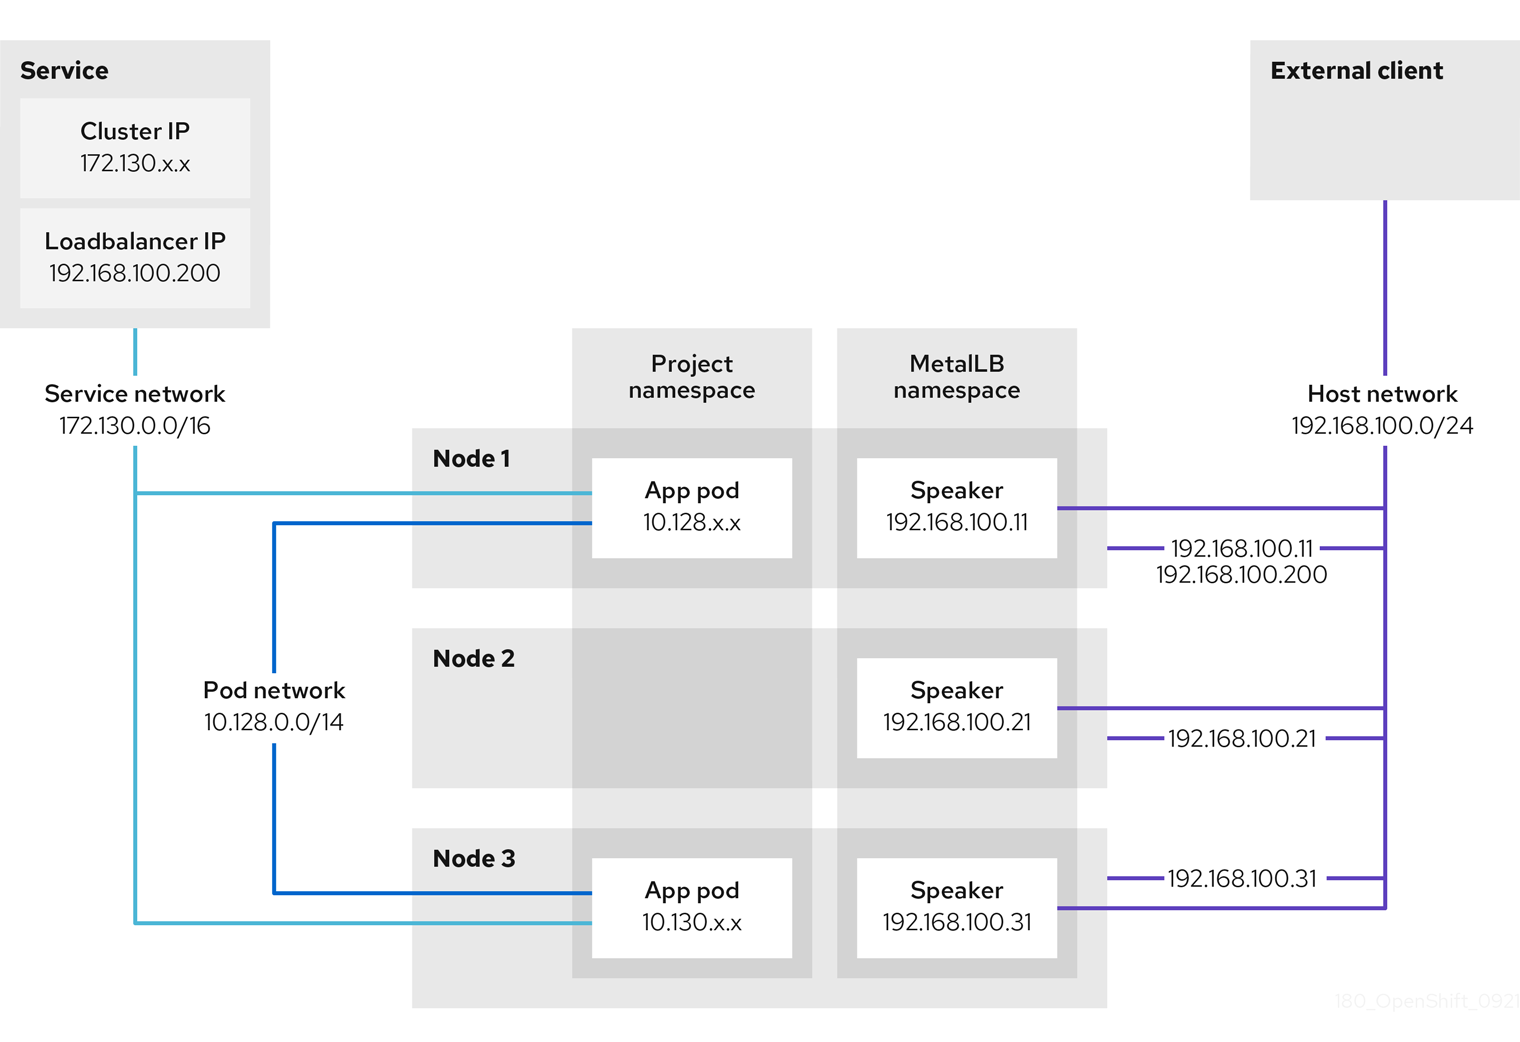
\includegraphics[width=0.8\textwidth]{\commonSecPathPrefix/../img/metallb-architecture.png}
    \caption{Архитектура и основные компоненты \textit{MetalLB} в режиме \textit{L2 LoadBalancer}}
    \label{fig:metallb-architecture}
\end{figure}

После запуска подов \textit{MetalLB} в кластере и объявления пула \textit{IP}-адресов, контроллер отслеживает создание сервисов с соответствующим типом и распределяет доступные адреса между ними, обеспечивая доступность извне.

\subsection{Установка и настройка модуля мониторинга}

Модуль мониторинга обеспечивает комплексный сбор, хранение, визуализацию и оповещение по метрикам и логам, что позволяет эффективно контролировать состояние и производительность кластера \textit{Kubernetes} и развернутых в нём приложений. В основе решения лежит интеграция нескольких специализированных компонентов, каждый из которых отвечает за определённую задачу мониторинга.

В состав модуля входят следующие компоненты:

\begin{itemize}
    \item \textit{VictoriaMetrics}\cite{victoriametrics} -- масштабируемая система сбора и хранения метрик с поддержкой \textit{Prometheus API};
    \item \textit{Grafana} -- платформа для визуализации метрик и построения дашбордов;
    \item \textit{Loki}\cite{loki} -- система централизованного хранения и поиска логов;
    \item \textit{Promtail} -- агент для сбора логов и передачи их в \textit{Loki};
    \item \textit{Alertmanager} -- компонент для управления оповещениями и их маршрутизации.
\end{itemize}

Все компоненты развёртываются в отдельном пространстве имён \textit{monitoring} с помощью инструмента \textit{FluxCD}, что обеспечивает автоматизацию, согласованность и лёгкость обновления конфигураций.

На рисунке~\ref{fig:monitoring-architecture} представлена архитектурная схема модуля мониторинга, иллюстрирующая взаимодействие компонентов, потоки данных метрик и логов, а также механизм оповещений.

\begin{figure}[ht]
    \centering
    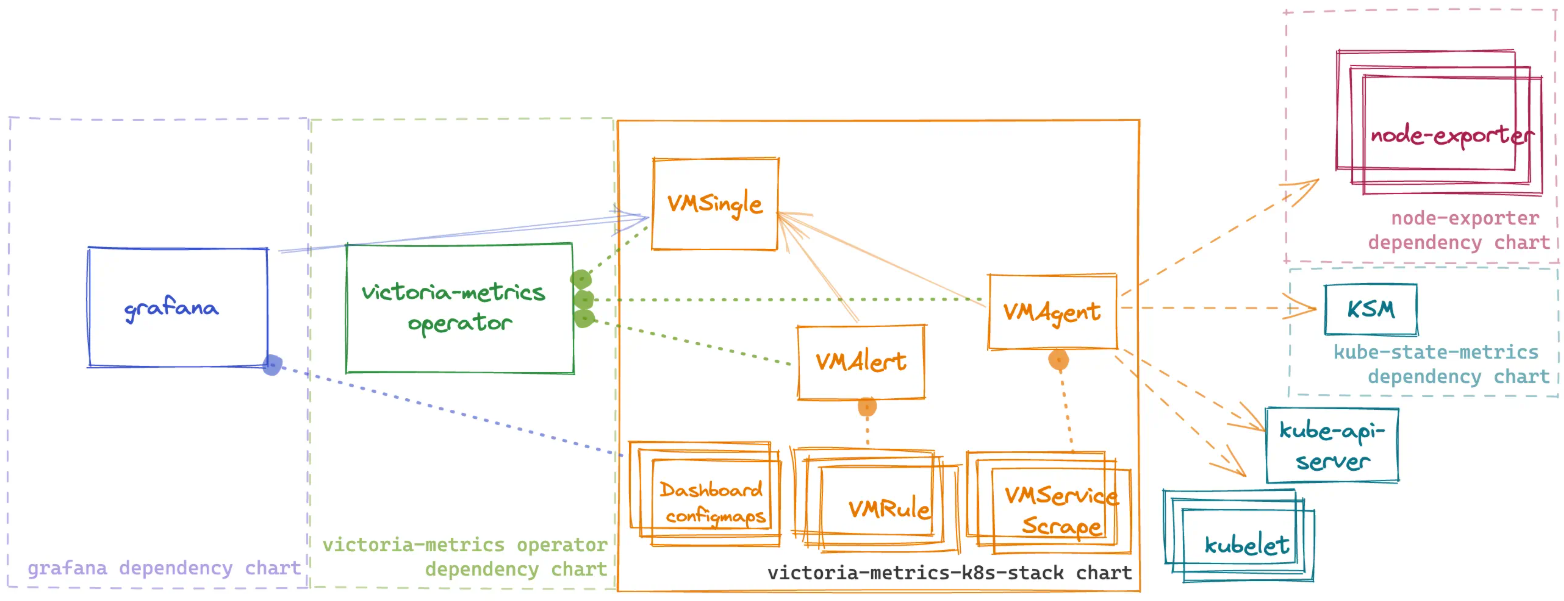
\includegraphics[width=0.9\linewidth]{\commonSecPathPrefix/../img/monitoring-architecture.png}
    \caption{Архитектура модуля мониторинга на базе \textit{VictoriaMetrics, Grafana, Loki, Promtail} и \textit{Alertmanager}}
    \label{fig:monitoring-architecture}
\end{figure}

\subsubsection{Добавление репозиториев \textit{Helm}.} Добавляются два источника \textit{Helm}-чартов:

\begin{itemize}
    \item \textit{https://victoriametrics.github.io/helm-charts} -- для установки стека \textit{VictoriaMetrics}, обновляемый каждые 24 часа;
    \item \textit{https://grafana.github.io/helm-charts} -- для установки систем \textit{Loki} и \textit{Promtail}, также обновляемый каждые 24 часа.
\end{itemize}

\subsubsection{Установка стека \textit{VictoriaMetrics}.} Установка производится с помощью ресурса \textit{HelmRelease}. Используется чарт \textit{victoria-metrics-k8s-stack} из ранее добавленного репозитория. Интервал обновления -- 30 минут. Конфигурация включает следующее:

\begin{itemize}
    \item отключены компоненты \textit{kubeEtcd}, \textit{kubeScheduler}, \textit{kubeControllerManager};
    \item включён компонент \textit{vmagent} с лимитом ресурсов: \textit{2560Mi} памяти и \textit{256m} \textit{CPU};
    \item компонент \textit{vmsingle} настроен с хранилищем объёмом \textit{4Gi}, периодом хранения данных в \textit{2 недели} и ограничением памяти \textit{700Mi};
    \item компонент \textit{Grafana} развёрнут с авторизацией через \textit{GitHub OAuth}, интерфейс доступен по адресу \textit{https://olymp.bsuir.by/i/grafana}, выставлены лимиты ресурсов: до \textit{400Mi} памяти и \textit{100m} \textit{CPU};
    \item добавлен сбор собственных метрик \textit{Grafana} с помощью \textit{vmScrape};
    \item загружаются два дашборда: \textit{NGINX} и \textit{Cloud Native PG} с помощью ресурсов \textit{ConfigMap}.
\end{itemize}

На рисунке~\ref{fig:vmstack-architecture} показана архитектура стека \textit{VictoriaMetrics}, отражающая взаимодействие компонентов и их основные ресурсы.

\begin{figure}[ht]
    \centering
    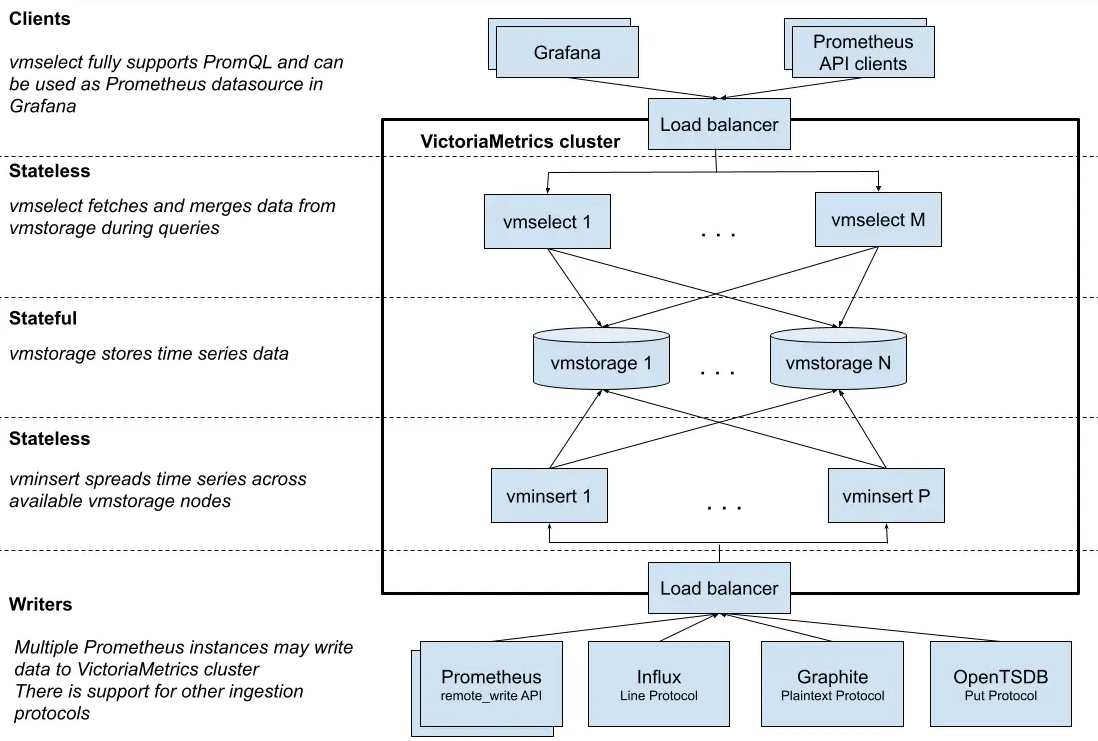
\includegraphics[width=0.9\linewidth]{\commonSecPathPrefix/../img/vm-arch.png}
    \caption{Архитектура стека \textit{VictoriaMetrics}}
    \label{fig:vmstack-architecture}
\end{figure}

\subsubsection{Настройка \textit{Alertmanager}.} Конфигурация \textit{Alertmanager} включает шаблоны для уведомлений в \textit{Telegram}, использующие форматирование и эмодзи. Уведомления включают ссылку на интерфейс \textit{Grafana}.

\subsubsection{Интеграция с системой оповещений \textit{FluxCD}.} Настроены три ресурса типа \textit{Alert}, обрабатывающие события от \textit{HelmRelease}, \textit{HelmRepository}, \textit{GitRepository} и \textit{Kustomization}. Уведомления отправляются в:

\begin{itemize}
    \item \textit{Telegram} -- для событий уровня \textit{info} и \textit{error};
    \item \textit{GitLab} -- для отображения статуса \textit{CI/CD}-процесса.
\end{itemize}

\subsubsection{Развёртывание \textit{Loki}.} Компонент \textit{Loki} развёрнут с использованием чарта \textit{loki} из официального репозитория \textit{Grafana}. Хранение логов настроено через \textit{S3}-совместимое хранилище, размещённое по адресу \textit{fksis-storage-01.bsuir.by}. Указан регион \textit{eu-west-1}, включена поддержка компакции и удаления старых данных с периодом хранения 672 часа.

\subsubsection{Развёртывание \textit{Promtail}.} Компонент \textit{Promtail} используется для сбора логов с узлов кластера и их отправки в \textit{Loki}. Подключение осуществляется через сервис \textit{loki-gateway}.

\subsubsection{Источники данных в \textit{Grafana}.} Создан ресурс \textit{ConfigMap} с конфигурацией источника данных типа \textit{Loki}, который автоматически подхватывается \textit{Grafana}.

В рамках данного раздела были разработаны программные модули, обеспечивающие автоматизированное развертывание и конфигурацию компонентов системы. Каждый модуль оформлен в виде \textit{Helm}-чарта, что позволяет обеспечить повторяемость, масштабируемость и удобство сопровождения инфраструктуры.

Для управления зависимостями и конфигурацией использованы возможности \textit{Helm}, такие как шаблоны, параметры значений и механизмы обновления. Модули обеспечивают корректную инициализацию сервисов, настройку доступа, а также безопасную работу с чувствительными данными.

\subsection{Настройка сервера \textit{OpenVPN}}

Сервер \textit{OpenVPN} обеспечивает безопасный удалённый доступ к корпоративной сети через защищённый туннель. В данном решении используется \textit{PKI} инфраструктура, реализованная через \textit{Vault PKI} для автоматического получения и обновления сертификатов, что значительно упрощает управление криптографическими материалами и повышает уровень безопасности.

\textit{OpenVPN} конфигурируется для работы на порту 1194 с использованием протоколов \textit{UDP} и \textit{UDP6}, что позволяет поддерживать как \textit{IPv4}, так и \textit{IPv6} подключение клиентов. Для организации \textit{VPN}-туннеля применяется виртуальный сетевой интерфейс типа \textit{tun}, который работает на уровне сетевого слоя, обеспечивая \textit{IP}-туннелирование.

\begin{lstlisting}
port 1194
proto udp
proto udp6

dev tun
\end{lstlisting}

Криптографические материалы -- сертификаты, ключи и параметры Диффи-Хеллмана -- хранятся в каталоге \textit{mutex\_gw\_legacy} и подгружаются сервером для установления защищённых соединений:

\begin{lstlisting}
ca        mutex_gw_legacy/ca.crt
cert      mutex_gw_legacy/server.crt
key       mutex_gw_legacy/server.key
dh        mutex_gw_legacy/dh.pem
tls-crypt mutex_gw_legacy/ta.key 0
\end{lstlisting}

Для адресации \textit{VPN}-клиентов выделена подсеть \textit{IPv4} \textit{10.8.0.0/24} и подсеть \textit{IPv6} \textit{2a01:4f9:c012:248d:80::/112}, что позволяет клиентам получать \textit{IP}-адреса из этих диапазонов:

\begin{lstlisting}
server 10.8.0.0 255.255.255.0
server-ipv6 2a01:4f9:c012:248d:80::/112
\end{lstlisting}

Для сохранения соответствия между клиентами и выданными им \textit{IP}-адресами используется файл \textit{ipp.txt}, что облегчает администрирование и мониторинг:

\begin{lstlisting}
ifconfig-pool-persist ipp.txt 0
\end{lstlisting}

Сервер автоматически передаёт клиентам маршруты к подсетям корпоративной сети, чтобы обеспечить корректный доступ к внутренним ресурсам:

\begin{lstlisting}
push "route 10.9.0.0 255.255.255.0"
push "route 192.168.0.0 255.255.240.0"
push "route-ipv6 2a01:4f9:c012:248d::/64"
\end{lstlisting}

Для корректного разрешения имён сервер дополнительно передаёт клиентам настройки \textit{DNS}, используя публичные \textit{DNS}-серверы \textit{Google}:

\begin{lstlisting}
push "dhcp-option DNS 8.8.8.8"
push "dhcp-option DNS 8.8.4.4"
\end{lstlisting}

В конфигурации включены дополнительные параметры, повышающие безопасность и устойчивость работы \textit{VPN}:

\begin{lstlisting}
client-to-client
duplicate-cn
keepalive 10 120

auth SHA512
cipher AES-256-GCM

persist-key
persist-tun

status openvpn-status.log
log         openvpn.log
log-append  openvpn.log
verb 3
explicit-exit-notify 1
\end{lstlisting}

Для удобства управления сервером включён интерфейс управления через \textit{UNIX}-сокет с использованием файлов аутентификации, а также поддержкой опциональной внешней авторизации и генерации токенов:

\begin{lstlisting}
management /run/openvpn-server/server.sock unix /etc/openvpn/password.txt
management-hold
management-client-auth
auth-user-pass-optional
auth-gen-token 28800 external-auth
\end{lstlisting}

Данная конфигурация обеспечивает надёжную, масштабируемую и безопасную работу \textit{OpenVPN} сервера с поддержкой \textit{IPv4} и \textit{IPv6}, автоматическим управлением сертификатами через \textit{Vault PKI} и гибкими настройками маршрутизации и аутентификации.

\subsection[ Настройка программного маршрутизатора \textit{Bird}]{Настройка программного маршрутизатора \textit{Bird}}

Для организации маршрутизации внутри корпоративной сети и обеспечения взаимодействия с \textit{VPN}-соединениями используется программный маршрутизатор \textit{Bird}. Он позволяет гибко управлять маршрутами и поддерживает протоколы динамической маршрутизации, такие как \textit{BGP}. Конфигурация \textit{Bird} обеспечивает интеграцию с системными таблицами маршрутизации, настройку статических маршрутов для \textit{VPN} и настройку \textit{BGP}-сессий с клиентами.

\begin{lstlisting}
log syslog all;
log "/var/log/bird.log" all;
\end{lstlisting}

В данной части конфигурации настраивается логирование. Все события маршрутизатора отправляются в системный журнал (\textit{syslog}), а также дублируются в файл \lstinline{/var/log/bird.log}. Это позволяет централизованно собирать логи и удобно отслеживать состояние работы маршрутизатора.

\begin{lstlisting}
router id 10.9.0.1;
\end{lstlisting}

Здесь задаётся уникальный идентификатор маршрутизатора в виде \textit{IP}-адреса, который используется в протоколах маршрутизации, например, \textit{BGP}, для идентификации устройства в сети.

\begin{lstlisting}
protocol kernel {
    ipv4 {
        import none;
    };
}
\end{lstlisting}

Данный блок описывает интеграцию с таблицей маршрутизации ядра операционной системы для \textit{IPv4}. Параметр \lstinline{import none} означает, что маршруты из системной таблицы не будут автоматически импортироваться в \textit{Bird}, что помогает избежать конфликтов и дублирования маршрутов.

\begin{lstlisting}
protocol device {}
\end{lstlisting}

Протокол \textit{device} отвечает за отслеживание состояния сетевых интерфейсов. Он обновляет маршруты при изменении статуса интерфейсов, что обеспечивает актуальность маршрутизации в динамичной сети.

\begin{lstlisting}
protocol static {
    ipv4;
    include "/etc/bird/sanctions_*";
    route 10.8.0.0/24 via "wg0";
    route 10.9.0.0/24 via "wg0";
}
\end{lstlisting}

В этом блоке задаются статические маршруты. Включение файлов из каталога \lstinline|/etc/bird/sanctions_*| позволяет реализовать фильтрацию или блокировку определённых маршрутов. Маршруты к подсетям \textit{VPN} (10.8.0.0/24 и 10.9.0.0/24) направляются через интерфейс \lstinline{wg0}, обеспечивая корректную маршрутизацию \textit{VPN}-трафика.

\begin{lstlisting}
template bgp MutexBgpRR {
    local as 65001;
    neighbor as 65001;
    capabilities off;
    ipv4 {
        export all;
    };
}
\end{lstlisting}

Этот шаблон определяет общие настройки для \textit{BGP}-сессий с клиентами. Локальный и соседний автономные номера систем (\textit{ASN}) заданы как 65001. Отключение дополнительных возможностей \textit{BGP} (\lstinline{capabilities off}) повышает совместимость. Все маршруты \textit{IPv4} экспортируются в соседа.

\begin{lstlisting}
protocol bgp client20 from MutexBgpRR {
    neighbor 10.9.0.20;
}

protocol bgp client21 from MutexBgpRR {
    neighbor 10.9.0.21;
}
\end{lstlisting}

На основе шаблона создаются две \textit{BGP}-сессии с клиентами, имеющими \textit{IP}-адреса 10.9.0.20 и 10.9.0.21 соответственно. Это позволяет обмениваться маршрутной информацией и динамически обновлять таблицы маршрутизации с этими узлами.

Таким образом, описанная конфигурация \textit{Bird} обеспечивает централизованное управление маршрутами с учётом особенностей \textit{VPN} и динамическую маршрутизацию через \textit{BGP}, что обеспечивает масштабируемость и устойчивость сети.
